\section{Beam and Detector}

The T2K experiment \citep{t2k-expt} is composed of a neutrino beamline
and a near detector at the J-PARC laboratory in Tokai, Japan, and
the far detector Super-Kamiokande (SK) situated \mbox{295 km} away in the Kamioka mine. 
The J-PARC accelerator complex produces a 30 GeV energy proton beam with spills
every 2.48 s that contain eight beam bunches which are 580 ns apart.
At this spill and repetition rate, 
a beam power of 430 kW
produces $2.25\times 10^{14}$ protons on target (PoT) per spill
corresponding to $\approx 0.8\times 10^{19}$ PoT integrated 
per day of data taking.

The proton beam
strikes a graphite target to produce pions and kaons that are focused
by three magnetic horns into a 96 m long decay pipe. The polarity of the magnetic horns
can be changed to Forward Horn Current (FHC) or Reverse
Horn Current (RHC) to select either positive or negative pions and
kaons to produce a predominantly $\nu_\mu$ or an $\bar\nu_\mu$ beam.
%
%The beamline direction produces a 2.5$^{\circ}$ off-axis \nuovernubar beam
%to SK whose \nuovernubar energy peaks at \textasciitilde{}0.6
%GeV. 
%
The resulting main neutrino beam axis is parallel to the proton beam direction. 
SK lies 2.5$^\circ$ off-axis with respect to the
main neutrino beam direction and this arrangement produces at SK both
the $\nu_\mu$ and $\bar\nu_\mu$ energies that peak at $\sim$0.6 GeV.
This $\nu_\mu$($\overline\nu_\mu$) peak energy with a 295 km baseline distance,
produces an $\frac{L}{E}$ value that maximizes the $\nu_{e}$($\overline{\nu}_{e}$)
appearance rate and has a $\nu_{\mu}$($\overline{\nu}_{\mu}$) disappearance
that minimizes the $\nu_\mu$($\overline\nu_\mu$) rates at SK.

The ND280 \nuandnubar fluxes were determined by simulation
of the T2K neutrino beamline \citep{t2k-flux} using 
FLUKA2011 \citep{fluka}, 
GEANT \citep{geant},
and GCALOR \citep{gcalor} 
software packages. The simulated hadronic yields have been re-weighted
using the %2016 
NA61/SHINE \citep{shine} thin-target data,
which has reduced the flux uncertainties to less than 10\% around the flux peak.
%and this reduced flux
%a factor 2 smaller from previous 2011
%uncertainties to less than 10\% below the peak energy 0.6 GeV. 
Detailed
descriptions of the ND280 flux uncertainties have been published in
previous ND280 analyses \citep{tpc-analysis-paper}. 
%The flux simulations
%provide the FHC (RHC) flux rates given in $\nu_{\mu}/\overline{\nu}_{\mu}/\nu_{e}/\overline{\nu}_{e}$
%( $\overline{\nu}_{\mu}/\nu_{\mu}/\overline{\nu}_{e}/\nu_{e}$ ) flavors
%n 11/5/7/2 (11/5/7/2) energy bins from 0 to 30 GeV and a
%$50\times50$ covariance matrix including neutrino and antineutrino
%correlations which is used to calculate systematic cross section uncertainties
%caused by these flux uncertainties. 
The typical fractional covariance
error of the T2K \nuandnubar fluxes are $\sim$10\%
and the $\nu_\mu$-$\bar\nu_\mu$ correlated flux errors are $\sim$6\%.
%The neutrino and antineutrino beam integrated rate is given in terms
%Protons on Target (PoT). 
%A beam power of 430 KW and a 2.48 second repetition
%spill rate, produces $2.25\times 10^{14}$ PoT per bunch which corresponds
%to $0.78\times 10^{19}$ PoT  per day.
The \nuandnubar flux rates
per cm$^{2}$/50 MeV/$10^{21}$ PoT are plotted in Fig.\ref{fig:The-neutrino-FHC}
with superimposed neutral lepton flavors, $\nu_\mu$,  $\nu_e$, $\bar\nu_\mu$ and $\bar\nu_e$.

The near detector complex, located 280m downstream of the target, consists
of an on-axis
detector (INGRID) and the ND280 off-axis detector. %{\color{blue} 
ND280 is positioned 
inline between the neutrino beam target and SK.  
The ND280 detector consists of sub-detectors inside
the refurbished UA1/NOMAD magnet that operates at a 0.2 T magnetic
field whose direction is horizontal and perpendicular to the neutrino beam.
The ND280 sub-detectors include $\pi^0$ detector \citep{p0d-1} (P$\emptyset$D),
three tracking time projection chambers \citep{tpc} (TPC1,2,3), two
fine-grained detectors (FGD1,2) interleaved with TPC1,2,3, and an
electromagnetic calorimeter (ECAL), that encloses the P$\emptyset$D, TPC1-3
and FGD1-2 sub-detectors. 

The measurements in this paper used the P$\emptyset$D and the TPC
tracking sub-detectors in the ND280 detector complex. In our description,
the +Z direction is parallel to the neutrino beam direction, and the +Y direction
is vertically upwards. Previous descriptions of analyses using the P$\emptyset$D have been published \citep{pod-nue}.
We describe additional details relevant for the analysis presented in this paper.

The P$\emptyset$D is shown in Fig.\ref{fig:Side-view-schematic}.
This detector contains 40 scintillator module planes called P$\emptyset$Dules.
Each P$\emptyset$Dule has 134 horizontal and 126 vertical triangular scintillator bars. 
A wavelength
shifting fiber centered in each bar is readout on one end by a silicon photomultiplier.
%Hamamatsu Multi-pixel photon counter (also known as silicon photomultipliers or SiPM). 
The P$\emptyset$D dimensions are $2298\times2468\times2350$ mm$^{3}$\textemdash XYZ\textemdash with
a total mass of $\sim$1900 kg of water and 3570 kg of other materials (mainly
scintillator with thin layers of high density polyethylene plastic and brass
sheet). The target material mass is given in fractional amounts in
Table \ref{tab:Chemical-composition-of}. These P$\emptyset$Dules are formed
into 3 major sections. The water target region, is
the primary target in this analysis which has 26 P$\emptyset$Dules interleaved with
bags of water 2.8 cm thick and 1.3 mm brass sheets. 
%This forms the water target which 
The water bags are drainable to allow water target subtraction
measurements. The two other regions (called upstream and central ECALs)
are the upstream and downstream sections that each contain 7 P$\emptyset$Dules
and steel sheets clad with lead (4.9 radiation lengths). 
%These two sections form
%a veto region to isolate neutrino 
%nteractions that occur within the water
%target section.

\begin{table}
%table captions at  top
\caption{\label{tab:Chemical-composition-of}Chemical element composition of
P$\emptyset$D water target region by fraction of mass. }


\begin{tabular}{lcc}
\hline 
\hline
Element & Symbol & Fraction\tabularnewline 
\hline 
Hydrogen & H & 8.0\%\tabularnewline 
Carbon & C & 45.0\%\tabularnewline 
Oxygen & O & 29.9\%\tabularnewline 
Copper & Cu & 14.3\%\tabularnewline 
Chlorine & Cl & 1.1\%\tabularnewline 
Titanium & Ti & 0.1\%\tabularnewline 
Zinc & Zn & 1.6\%\tabularnewline
\hline
\hline 
\end{tabular}

\end{table}

\begin{figure}
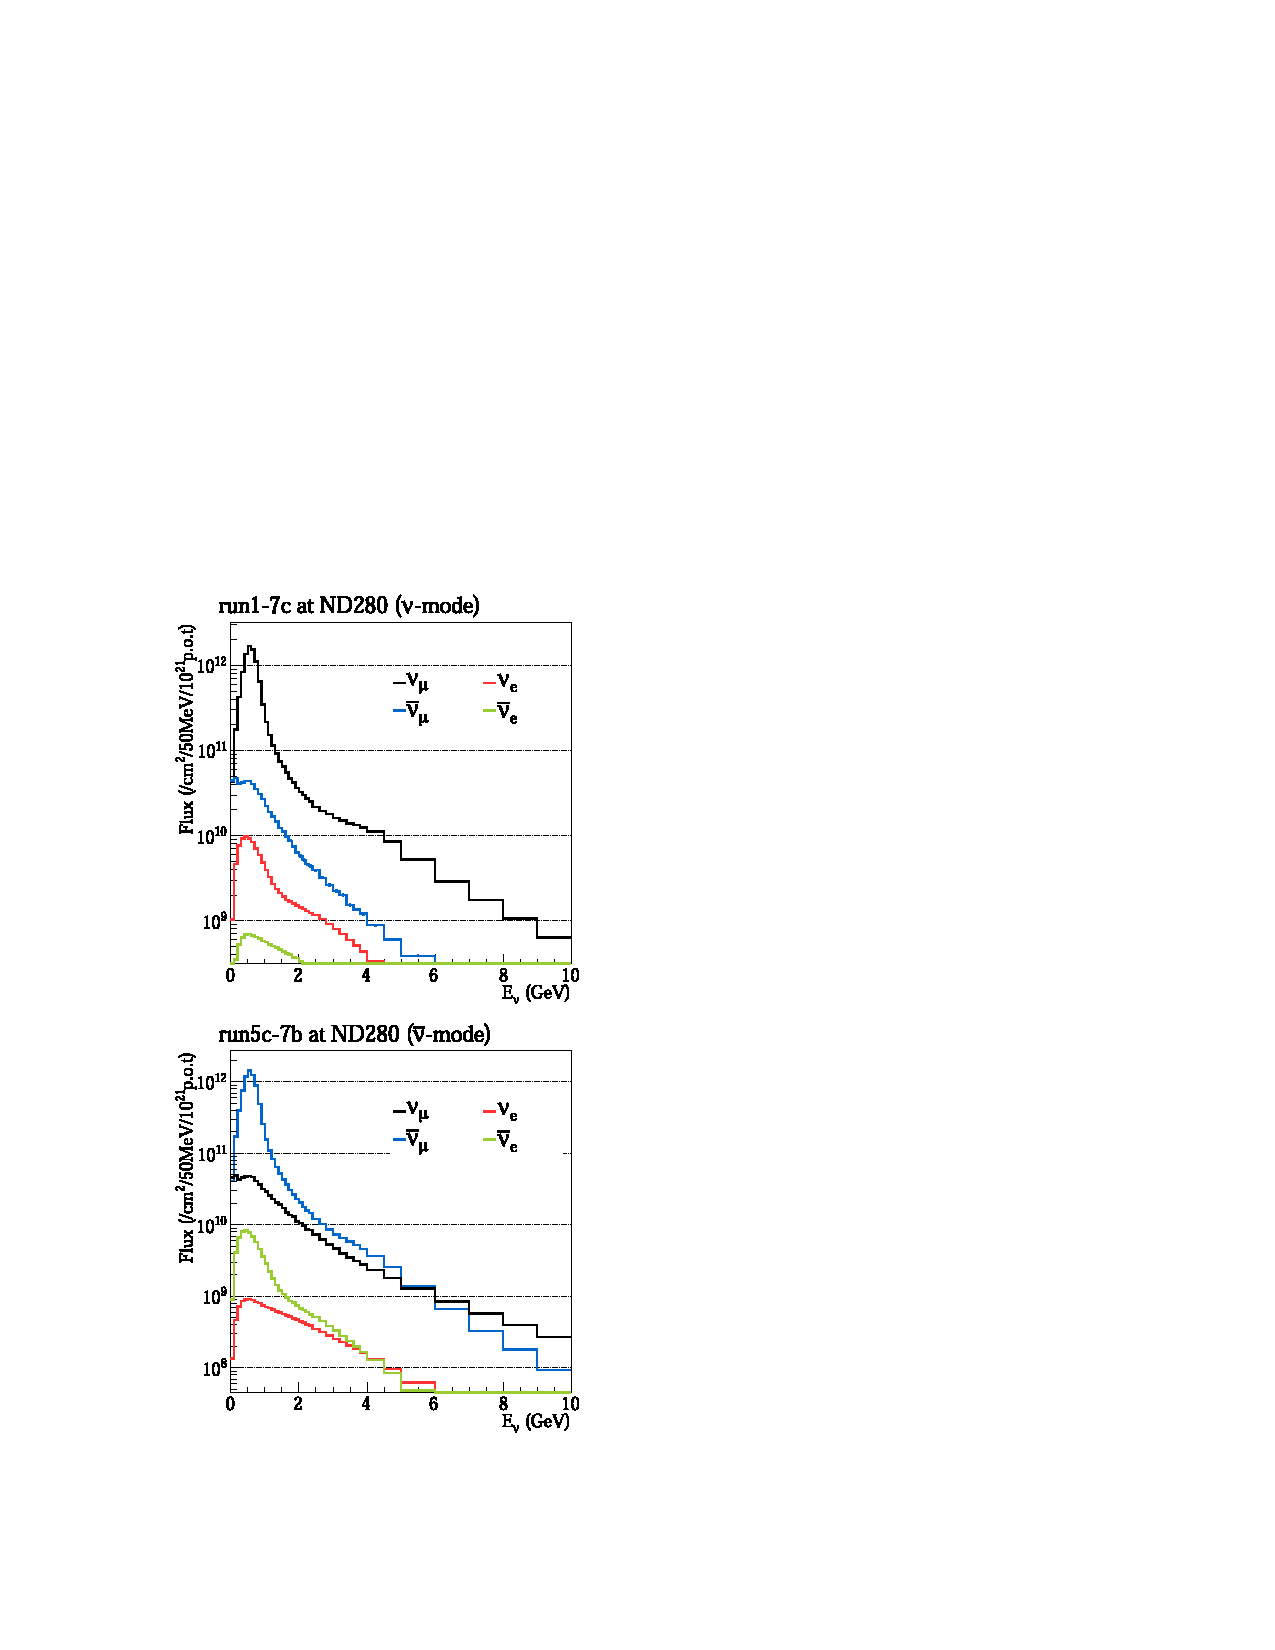
\includegraphics[scale=1.0]{flux2014-v8-both} 
\caption{\label{fig:The-neutrino-FHC}The predominately neutrino FHC beam (Top) and 
predominately antineutrino
RHC beam (Bottom) flux per PoT as a function of energy
at the ND280 detector. The rates are separated by neutrino/antineutrino
muon and electron type flavors. The peak values for the neutrino and
the antineutrino flux rates are $1.7\times10^{12}$ and $1.4\times10^{12}$
/cm$^{2}$/50MeV/10$^{21}$ PoT, respectively.}
\end{figure}

\begin{figure}
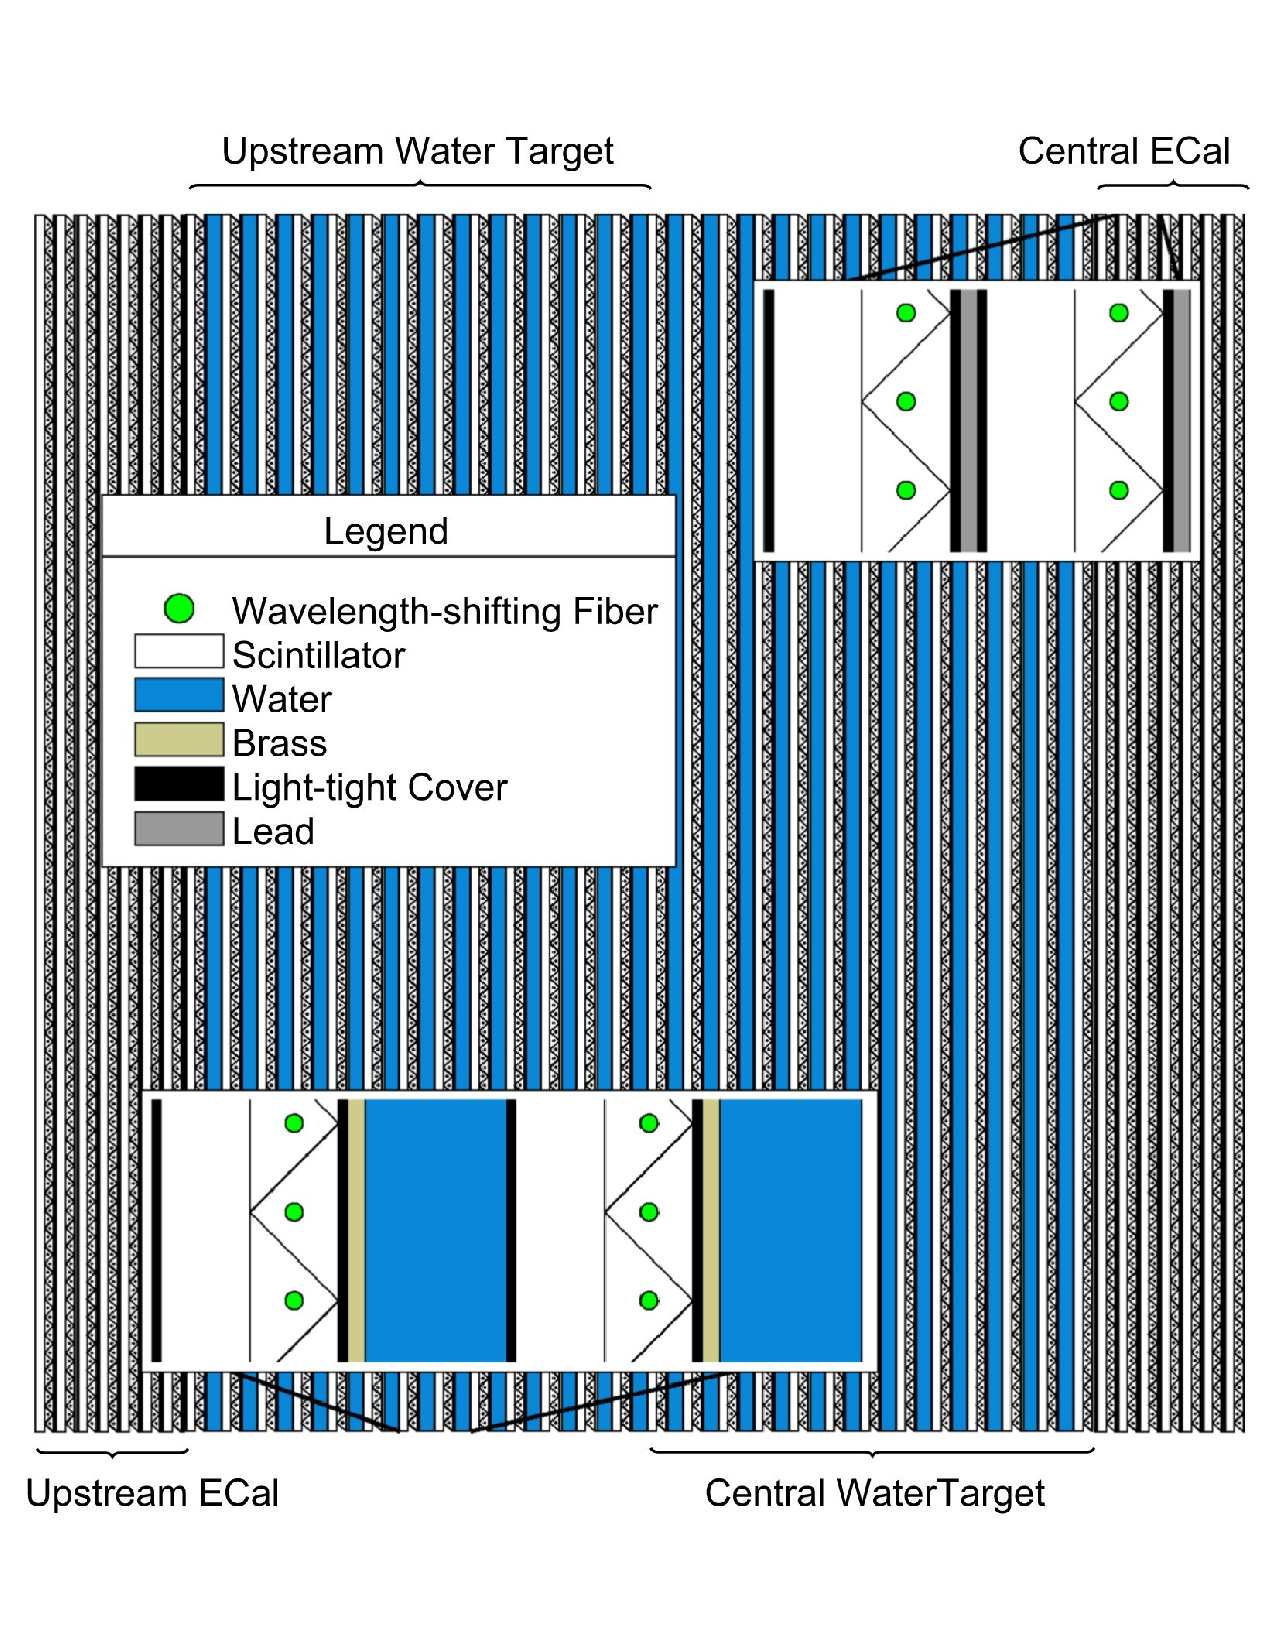
\includegraphics[scale=0.4]{P0D-crop}
%{P0D-diagram.JPG}

\caption{\label{fig:Side-view-schematic}Side view schematic diagram of the
P$\emptyset$D detector. The white, zig-zag, and blue strip regions represent
the vertical scintillator bars, the horizontal scintillator bars,
and the water bag regions, respectively. The vertical and horizontal
bars represent a X-Y module or P$\emptyset$Dule. The first and last groups of
seven P$\emptyset$Dules form the upstream and the central ECAL ``super'' modules
and the middle 26 P$\emptyset$Dules interleaved with the water bags are the
water target region.}
\end{figure}

The TPC1,2,3 detectors are three modules whose dimensions are each
$1808\times2230\times852$ mm$^{3}$\textemdash XYZ\textemdash where each module
contains a centered high voltage (Z-Y)
cathode plane that splits the chamber into two sections where the charged particle track ionizations drift
in the $\pm X$ directions. These are measured by 70~mm$^{2}$ micromegas
pads in the Z-Y plane. The fully contained ionized track path
lengths are 72 cm. A charged track will be measured with $\sim$0.7
mm resolution for drift distances >10 cm.
% and this provides dE/dX measurements
%that have $>4\sigma$ particle ID separation between electrons and
%muons in the momentum range $200<p<300$ MeV/c. 
The typical
TPC momentum resolution is $\delta\left(p_{\bot}\right)/p_{\bot}=0.08p_{\bot}$ (GeV/c). 
Analyses which use the TPC have been
described in previous ND280 publications \citep{tpc-analysis-paper}.

%This analysis utilized data taken for both beam polarities. The neutrino
%beam mode data was taken from February 2013 to August 2013 for a total
%exposure of $16.24\times10^{19}$ PoT. The anti-neutrino beam mode
%data was taken from May 2014 through June 2014 for an exposure of
%$4.30\times10^{19}$ PoT. These integrated rates corresponds to roughly
%$0.28\times10^{12}$ neutrinos and $0.06\times10^{12}$ antineutrinos
%per cm$^{2}$-50 MeV at 0.6 GeV/c$^{2}$. 


